\documentclass[compress,red]{beamer}

%\documentclass[c,10pt,dvips]{beamer}
%\documentclass[c,11pt,dvips,handout]{beamer}

\usepackage[utf8]{inputenc}                 %%% UTF8 kódování češtiny
%\usepackage[cp1250]{inputenc}              %%% kódování češtiny běžné v MS Windows

%\usepackage[english]{babel}
%\usepackage{czech}                                 %%% jedna z možností, jak nastavit češtinu

\usepackage[czech]{babel}                           %%% druhá možnost, jak nastavit češtinu
%\ifx\uv\undefined\newcommand{\uv}[1]{,,#1``}\fi     %%% příkaz pro sazbu českých/slovenských uvozovek
                                                    %%% (v novějších verzích babelu je již k dispozici, stejně tak je již k dispozici v balíčku czech)

\usepackage{pgfpages}
%\pgfpagesuselayout{2 on 1}[a4paper, border shrink=5mm]              %%% k použití tvorby poznámek (2 slidy, resp. 4 slidy na stránce)
%\pgfpagesuselayout{4 on 1}[a4paper, landscape, border shrink=5mm]


%%%%% Několik užitečných balíčků
%%%%% ----------------------------------------------------------
\usepackage{helvet}                 %%% font
\usepackage{amsmath, amssymb}       %%% matematické symboly
\usepackage{multicol}               %%% vícesloupcová sazba
\usepackage{graphicx, fancybox}     %%% vkládání obrázků
\usepackage{psfrag}                 %%% dodatečná úprava popisků v postscriptech
\usepackage{fancyvrb}               %%% vylepšené prostředí pro strojové písmo
\usepackage{bbding}                 %%% hezké symboly
\usepackage{comment}

\usepackage{subfigure}
\usepackage{epsfig}
%\usepackage[all,knot]{xy}
%\xyoption{arc}
\usepackage{url}
\usepackage{multimedia}
\usepackage{hyperref}
\usepackage{setspace}
\usepackage{epstopdf}
%\usepackage{breqn}
\usepackage{amsmath}
\usepackage{tikz}
\DeclareGraphicsExtensions{.pdf,.eps,.png,.jpg,.mps}


%%%%% Definice několika barev
%%%%% ----------------------------------------------------------
\definecolor{redmff}{rgb}{0.7892720,0.0651341,0.1455939}          % Pantone 186, oficiální červená barva MFF UK

\definecolor{darkblue}{rgb}{0,0,0.3}
\definecolor{bcred}{rgb}{1,0,0}
\definecolor{bcblue}{rgb}{0,0,0.7}
\definecolor{bcwhite}{gray}{0.98}
\definecolor{bcgray}{gray}{0.92}

\definecolor{colOne}{rgb}{0,0,0}        %% barva první úrovně
\definecolor{colTwo}{rgb}{0,0,0.3}      %% barva druhé úrovně


%%%%% Nastavení balíčku beamer
%\usetheme{Warsaw}
% other themes: AnnArbor, Antibes, Bergen, Berkeley, Berlin, Boadilla, boxes, CambridgeUS, Copenhagen, Darmstadt, default, Dresden, Frankfurt, Goettingen,
% Hannover, Ilmenau, JuanLesPins, Luebeck, Madrid, Maloe, Marburg, Montpellier, PaloAlto, Pittsburg, Rochester, Singapore, Szeged, classic

%\usecolortheme{lily}
% color themes: albatross, beaver, beetle, crane, default, dolphin, dov, fly, lily, orchid, rose, seagull, seahorse, sidebartab, structure, whale, wolverine

%\usefonttheme{serif}
% font themes: default, professionalfonts, serif, structurebold, structureitalicserif, structuresmallcapsserif

% pdf is displayed in full screen mode automatically
%\hypersetup{pdfpagemode=FullScreen}

%\useoutertheme[subsection=false]{smoothbars}

%%%%% ----------------------------------------------------------
\mode<presentation> {
    \usetheme{Warsaw}                 %% jedno možné téma
    %\usetheme{CambridgeUS}           %% jiné možné téma

    \usecolortheme{beaver}            %% jedno možné téma pro barvy (stejně bude většina barev předefinována)
    %\usecolortheme{wolverine}

    %%%\setbeamercolor{background canvas}{bg=}                                                         %% odkomentuj, chceš-li použít soubor layout.eps (lze vyseparovat např. z PowerPointové prezentace) jako pozadí
    %%%\usebackgroundtemplate{\includegraphics[width=\paperwidth, height=\paperheight]{layout.eps}}    %% odkomentuj, chceš-li použít soubor layout.eps (lze vyseparovat např. z PowerPointové prezentace) jako pozadí

    %%% Předefinování některých barev, aby to pěkně ladilo mému oku a +- odpovídalo JGS MFF UK
    %%% -----------------------------------------------------------------------------------------
    \setbeamertemplate{background canvas}[vertical shading][bottom=bcwhite, top=white, middle=bcwhite!50!white]
    \setbeamercolor{background canvas}{bg=white}       %% NO EFFECT WHEN \setbeamertemplate{background canvas} WAS USED
    \setbeamercolor{frametitle}{fg=white, bg=redmff}   %% NO EFFECT on bg
    \setbeamercolor{normal text}{fg=black}
    \setbeamercolor{alerted text}{fg=redmff}
    \setbeamercolor{math text inlined}{fg=bcblue}
    \setbeamercolor{math text displayed}{fg=bcblue}
    \setbeamercolor{bcboxcol}{fg=darkblue, bg=bcgray}

    %%% Nastaví v matematice na patkové
    %\usefonttheme[onlymath]{serif}

    %%% Odrážky budou "hranaté" místo "kulatých"
    %\useinnertheme{rectangles}

    %%% Specifikuje co má být v hlavičce
    \setbeamertemplate{headline}{}

    %%% Obsah paty (jednoduché nastavení)
    %\setbeamercolor{page number in head/foot}{fg=black, bg=white}

    %%% Obsah paty (složitější nastavení)
    \setbeamertemplate{footline} {
      \hspace*{2.5em}
      \begin{beamercolorbox}{section in head/foot}
      \vskip1pt
      \textcolor{black}{\small \insertpagenumber}\hfill
      \textcolor{darkblue}{\scriptsize\hfill Martin Holeček\hfill %\texttt{komarek@karlin.mff.cuni.cz}
      }\hfill
      \textcolor{redmff}{\footnotesize Words learning using deep structures}
      \hspace*{3.5em}
      \vskip3pt
      \end{beamercolorbox}
    }

    %%% Vypíná zápatí s navigačními symboly
    %\setbeamertemplate{navigation symbols}{}

    %%% Levý a pravý okraj
    %\setbeamersize{text margin left=1cm}
    %\setbeamersize{text margin right=1cm}
}

%%%%% Logo na každé stránce
%\logo{\colorbox{white}{\includegraphics[height=1.5cm, width=1.5cm]{mff_logo.eps}}}


%%%%% Ukázka použití fancyvrb  (prostředí pro softwarový vstup a výstup)
%\newcommand{\Rko}{\includegraphics[width=5.094mm, height=3.876mm]{Rlogo.eps}}   %% R logo, original size is 8.49 x 6.46 mm
\DefineVerbatimEnvironment{Rin}{Verbatim}{formatcom=\color{bcred}, fontsize=\footnotesize, frame=single, framerule=1pt, framesep=1pt}
\DefineVerbatimEnvironment{Rout}{Verbatim}{formatcom=\color{bcblue}, fontsize=\footnotesize, frame=single, framerule=1pt, framesep=1pt}


%%%%% Beamer nastavení dokumentu
%%%%% ------------------------------------------------
\title[Words learning using deep structures]{%
      Words learning using deep structures}
%\subtitle{}

%\author{Martin Holeček}
%\institute[MFF UK v Praze]{Matematicko-fyzikální fakulta Univerzity Karlovy v~Praze}

\date[19.6.2015]{19.6.2015}


\begin{document}

\begin{comment}
%%%%% Titulní slide (udělaný ``ručně'')
% ---------------------------------------------------------------------------------------
\begin{frame}[plain]

%\vspace*{-0.5em}
\begin{center}
%\includegraphics[width=80mm, height=38mm]{mff_cz_color.eps}       %% logo MFF, original size is 100 x 44 mm
\-raphics[width=80mm, height=38mm]{mff_cz_color.eps}       %% logo MFF, original size is 100 x 44 mm

\bigskip
\textcolor{black}{\normalsize\bfseries Martin Holeček} \\[0.5ex]
\textcolor{black}{\small Obecná matematika}

\bigskip
%\textcolor{redmff}{\Large\bfseries SVOČ 2013} \\[0.5ex]
\textcolor{redmff}{\Large\bfseries Efektivní metody zobrazování objemových dat}

\bigskip
\textcolor{darkblue}{\small 22. května 2013}
\end{center}
\end{frame}


\end{comment}

%%%%% Automatický titulní slide
% ---------------------------------------------------------------------------------------
%%% Vyberte si pouze jeden způsob tvorby titulní stránky!!!
\begin{frame}[plain]
 \titlepage
\end{frame}


%%%%% Úvodní část
%%%%% ===================================================================================
\section{Into}    %%% Začátek úvodní části


%%%%% Slide
%
% 
% So lets refresh how we can represent text. Basically three approaches, the tree at the bottom is an example of grammatic model.
%
% ----------------------------------------------------------------------------------------
\begin{frame}\frametitle{Representatins of text}
\framesubtitle{Intro}
\begin{itemize}
\item Grammatical models
\item Bag of words
\item Vectorization and complex ideas
\end{itemize}
\begin{center}
\includegraphics[width=0.3\columnwidth]{engsyntx.png}
\end{center}

\end{frame}

%%%%% Slide
%
% BOW jsme meli na prednasce, zbyva jenom rict, ze se da pouzit i na bigramy, unigramy atp a co s nim pak lze delat
% there are even some attempts to use a  combination of bigrams or trigrams or to use BOW to see which words to filter and what preprocessing to do. How big is that? 300000 words squared on bigrams...
%
% ----------------------------------------------------------------------------------------
\begin{frame}\frametitle{BoW}
\framesubtitle{Intro}
\begin{itemize}
\item Forgets sequential information
\item Sparse
\item TF-IDF (Terms frequency, inverse document frequency)
\item unigrams / bigrams / trigrams
\item Latent dirichlet allocation
\item Latent semantic indexing
\end{itemize}
\begin{center}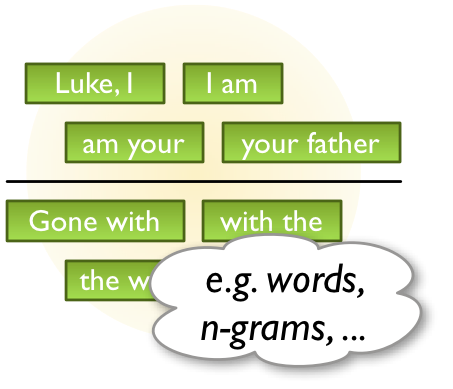
\includegraphics[width=0.4\columnwidth]{sally3.png}
\end{center}
\end{frame}

%%%%% Slide
%
%  2 ideas of vectorization
%
%
%
% ----------------------------------------------------------------------------------------
\begin{frame}\frametitle{Vectorization}
\framesubtitle{Intro}
\begin{itemize}
\item word2vec - assisted to group similar meanings
\item Text understanding from scratch
\end{itemize}
\begin{center}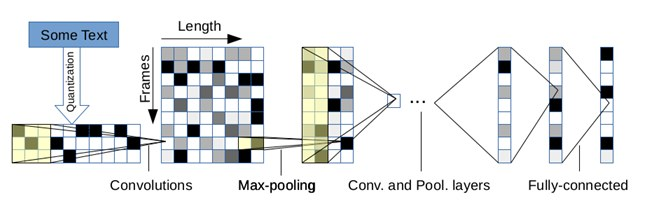
\includegraphics[width=1.0\columnwidth]{text-deep-learning.jpg}
\end{center}
\end{frame}

%%%%% Slide
%
% Usage - my original idea is to assign a diagnosis to a medical report text. For that, I believe, no gramatical model is usable
% and also I dont have a good computer for bag of words or for
%
%
% ----------------------------------------------------------------------------------------
\begin{frame}\frametitle{Usage}
\framesubtitle{Intro}
\begin{itemize}
\item Text classification (sentinent analysis, emotion recognition)
\item clustering (for indexing documents, for groupping similar texts)
\end{itemize}
\end{frame}

\section{Main}

%%%%% Slide
% ----------------------------------------------------------------------------------------
\begin{frame}\frametitle{The idea}


\begin{center}
"Gsues wichh of tshee tehre scenetens mghit be mroe rdbleaae?"

\begin{multline*}
r:\,\mathcal{A}^{\infty}\rightarrow\mathcal{B}\subset\mathbb{R}^{2\cdot|\mathcal{A}|}:\,word\in\mathcal{A}^{\infty}\rightarrow r(word)\in\mathcal{B}:\,r(word)= \\
( \sum_{c\in|\mathcal{A}|}vec(c)\cdot\sum_{i=0}^{len(word)}\delta_{vec(word_{[i]}),vec(c)}, \\  vec(word_{[0]})+vec(word_{[len(word)]}) )
\end{multline*} 

\begin{tikzpicture}
\def\blcknss{% 
   {0.0,0.0,0,0.0,0.125,0,0.125,0,%h
0,0,0,0,0,0,0,0,%p
0,0,0.250,0,0.125,0,0,0,%x
0,0,%z
0,0,0,0,0,0,0.5,0,%h
0,0,0,0,0,0,0,0,
0,0,0.5,0,0,0,0,0,
0,0}}% 
\draw[ultra thick] (0,0) rectangle (10,-10/52);
    \foreach \column in {0, ..., 51} {
     \fill[fill=black, opacity={\blcknss[ \column ]} ] ({\column/52*10},0)   rectangle +(10/52,-10/52);
      %  \foreach \column in {0, ..., 52} {
   % \fill ({2*\column + mod(\row,2)}, -\row) rectangle +(10/52,-10/52);
     %   }
 }
\end{tikzpicture}	

\end{center}

\end{frame}

%%%%% Slide
%
% this idea comes from the sentence. these words should be hard to read near each other.
%The representation is more or less unique and also if you do remember how small childern try to read in basic schools
% it is the same - they often mistake words based on beginning and ending character.
% yes, there is also an idea to drop a,e,i,o,u and still able to read it, but then it might not be that much unique
% somebody tried to make this idea even more applied and teaches speedreading as first and last word in a paragraph and the words in between.
%
%
% ----------------------------------------------------------------------------------------
\begin{frame}\frametitle{Justification}
\framesubtitle{The idea}

\begin{itemize}
\item doorstops doorposts 
\item doorstops doorposts 
\item kleig klieg 
\item noncasual noncausal 
\item organization's organizations
\item regains reginas
\item snakes sneaks 
\item teazles teazels 
\end{itemize}
(To try another language - from a Czech dictionary consisting of 300000 words, the number of collisions are 43.)
\end{frame}

%%%%% Slide
% ----------------------------------------------------------------------------------------
\begin{frame}\frametitle{Properties}
\framesubtitle{The idea}

\begin{itemize}
\item VS Gramatic models - different plugins for different languages
\item VS bag of words - big input space
\item every word has a fixed length
\item mostly sparse 
\item to reconstruct the word from its code
\item humans system
\end{itemize}
\end{frame}

%%%%% Slide
%
%
% Notice that nobody paint the autoencoder with the bias unit. Moving window, convolutionals are on the slide before
%
% ----------------------------------------------------------------------------------------
\begin{frame}\frametitle{Architectures tried and to try}

\begin{itemize}
\item autoencoders
\item convolutional neural networks
\item Moving window
\item (RBM)
\item (RBM + autoenc)
\end{itemize}

\begin{center}
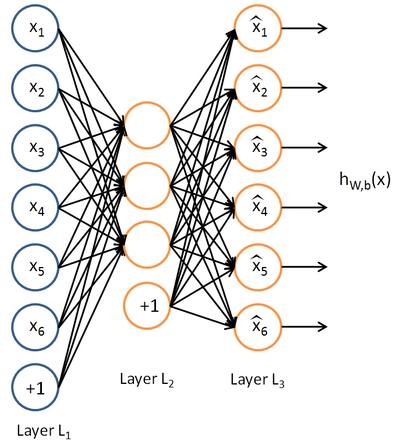
\includegraphics[width=0.3\columnwidth]{400px-Autoencoder636.png}
\end{center}


\end{frame}

%%%%% Slide
%
% about dbpedia
% DBpedia is something I wanted to test it on, because 
% 
%
%
% ----------------------------------------------------------------------------------------
\begin{frame}[fragile]\frametitle{Datasets tried}
\begin{itemize}
\item orders (failed)
\item DBpeadia
\end{itemize}
\end{frame}

%%%%% Slide
%
% how these work
%
%
% ----------------------------------------------------------------------------------------
\begin{frame}[fragile]\frametitle{some libraries for NNs}
\begin{itemize}
\item FANN
\item Theano
\item Pylearn2
\end{itemize}
\end{frame}

%%%%% Slide
% ----------------------------------------------------------------------------------------
\section{Experiments and results}
\begin{frame}\frametitle{Experiments}

\begin{itemize}
\item speed of 47 words
\item Learning rate 0.1, L2 regularization 0.0001
\item batch sizes were chosen to be 361, size of training dataset was 649800 and testing and validation sets 238260 items each.
\item smaller convNN: 20 frames+kernel 5x5+pool2x2; 30 frames+kernel 5x5+pool2x2; 20 frames+kernel 5x5+pooling2x2; 500 fully connected sigmoid.
\item larger convNN: 30 frames+kernel 5x5+pool2x2; 40 frames+kernel 5x5+pool2x2; 50 frames+kernel 5x5+pooling2x2; 1000 fully connected sigmoid.
\item autoencoder (sigmoid layers), number of neurons: 3000, 4000,3000,2000,1000,500,200,100
\end{itemize}
\end{frame}

%%%%% Slide
%
% So, first, the convolutional network. I did two sizes to see if the results will get better. They get.
% the other guy gets to 98% accuracy but with 1000 frames and 3 times more layers.
%
%
% ----------------------------------------------------------------------------------------
\begin{frame}\frametitle{It Works!}
\framesubtitle{ConvNN}

\begin{itemize}
\item 51.54\% validation error, 52.76\% test error for bigger convolutional network 
\item and 53.80\% validation, 55.23\% for smaller network on dbpeadia dataset 
\end{itemize}

\end{frame}

%%%%% Slide
% ----------------------------------------------------------------------------------------
\begin{frame}\frametitle{It Works!}
\framesubtitle{Autoencoder}

\begin{small}
"A Walk in the Sun is a World War II war film released in 1945 based on the novel by Harry Brown who was a writer for Yank the Army Weekly based in England..."

\begin{itemize}
%dist: 3.78E-05 
%"Dinglewood is a neighborhood/subdistrict located at the southern edge of Downtown Columbus Georgia. In it is the tallest building in Columbus the Aflac Tower. It is also home to the famous Dinglewood Pharmacy which serves in the opinions of the city's residents the city's best scrambled hot dog. The boundaries of the neighborhood are generally acknowledged to be 17th Street to the north Martin Luther King Jr."

\item "A Walk to Beautiful is a 2007 American documentary film produced and distributed by Engel Entertainment about women who suffer from childbirth injuries in Ethiopia. In 2007 it premiered in film festivals and was chosen for the International Documentary..." (dist: 2.94E-06 )

\item "A Walk in the Woods: Rediscovering America on the Appalachian Trail is a 1998 book by travel writer Bill Bryson describing his attempt to walk the Appalachian Trail with his friend Stephen Katz. The book is written..." (dist: 0 ) 
\end{itemize}

Some of the far-away (dist $>7$) :
\begin{itemize}
\item She Married for Love is a 1914 silent comedy film featuring Oliver Hardy.
\item The Scroafa River is a tributary of the Archita River in Romania.
\end{itemize}
\end{small}

\end{frame}


%%%%% Slide
% ----------------------------------------------------------------------------------------
\begin{frame}[plain]
%%% Rámeček
\begin{beamercolorbox}[center, sep=2pt, rounded=true, shadow=true]{bcboxcol}
\LARGE\bfseries Tkahns for aotnitten! \\
\end{beamercolorbox}
\end{frame}




\end{document}





